
%%%%%%%%%%%%%%%%%%%%%%%%%%%%%%%%%%%%%%%%%%%%%%%%%%%%%%%%%%%%%%%%%%%%%%%%%%%%%%%%%%%%%%%
%%%%%%%%%%%%%%%%%%%%%%%%%%%%%%%%%%%%%%%%%%%%%%%%%%%%%%%%%%%%%%%%%%%%%%%%%%%%%%%%%%%%%%%
% 
% This top part of the document is called the 'preamble'.  Modify it with caution!
%
% The real document starts below where it says 'The main document starts here'.

\documentclass[12pt]{article}

\usepackage{amssymb,amsmath,amsthm}
\usepackage[top=1in, bottom=1in, left=1.25in, right=1.25in]{geometry}
\usepackage{fancyhdr}
\usepackage{enumerate}
\usepackage{listings}
\usepackage{graphicx}
\usepackage{float}
% Comment the following line to use TeX's default font of Computer Modern.
\usepackage{times,txfonts}



\makeatletter
\renewcommand*\env@matrix[1][*\c@MaxMatrixCols c]{%
  \hskip -\arraycolsep
  \let\@ifnextchar\new@ifnextchar
  \array{#1}}
\makeatother

\newtheoremstyle{homework}% name of the style to be used
  {18pt}% measure of space to leave above the theorem. E.g.: 3pt
  {12pt}% measure of space to leave below the theorem. E.g.: 3pt
  {}% name of font to use in the body of the theorem
  {}% measure of space to indent
  {\bfseries}% name of head font
  {:}% punctuation between head and body
  {2ex}% space after theorem head; " " = normal interword space
  {}% Manually specify head
\theoremstyle{homework} 

% Set up an Exercise environment and a Solution label.
\newtheorem*{exercisecore}{Exercise \@currentlabel}
\newenvironment{exercise}[1]
{\def\@currentlabel{#1}\exercisecore}
{\endexercisecore}

\newcommand{\localhead}[1]{\par\smallskip\noindent\textbf{#1}\nobreak\\}%
\newcommand\solution{\localhead{Solution:}}

%%%%%%%%%%%%%%%%%%%%%%%%%%%%%%%%%%%%%%%%%%%%%%%%%%%%%%%%%%%%%%%%%%%%%%%%
%
% Stuff for getting the name/document date/title across the header
\makeatletter
\RequirePackage{fancyhdr}
\pagestyle{fancy}
\fancyfoot[C]{\ifnum \value{page} > 1\relax\thepage\fi}
\fancyhead[L]{\ifx\@doclabel\@empty\else\@doclabel\fi}
\fancyhead[C]{\ifx\@docdate\@empty\else\@docdate\fi}
\fancyhead[R]{\ifx\@docauthor\@empty\else\@docauthor\fi}
\headheight 15pt

\def\doclabel#1{\gdef\@doclabel{#1}}
\doclabel{Use {\tt\textbackslash doclabel\{MY LABEL\}}.}
\def\docdate#1{\gdef\@docdate{#1}}
\docdate{Use {\tt\textbackslash docdate\{MY DATE\}}.}
\def\docauthor#1{\gdef\@docauthor{#1}}
\docauthor{Use {\tt\textbackslash docauthor\{MY NAME\}}.}
\makeatother

% Shortcuts for blackboard bold number sets (reals, integers, etc.)
\newcommand{\Reals}{\ensuremath{\mathbb R}}
\newcommand{\Nats}{\ensuremath{\mathbb N}}
\newcommand{\Ints}{\ensuremath{\mathbb Z}}
\newcommand{\Rats}{\ensuremath{\mathbb Q}}
\newcommand{\Cplx}{\ensuremath{\mathbb C}}
%% Some equivalents that some people may prefer.
\let\RR\Reals
\let\NN\Nats
\let\II\Ints
\let\CC\Cplx

%%%%%%%%%%%%%%%%%%%%%%%%%%%%%%%%%%%%%%%%%%%%%%%%%%%%%%%%%%%%%%%%%%%%%%%%%%%%%%%%%%%%%%%
%%%%%%%%%%%%%%%%%%%%%%%%%%%%%%%%%%%%%%%%%%%%%%%%%%%%%%%%%%%%%%%%%%%%%%%%%%%%%%%%%%%%%%%
% 
% The main document start here.

% The following commands set up the material that appears in the header.
\doclabel{Math 614: Homework 1}
\docauthor{Stefano Fochesatto}
\docdate{\today}

\begin{document}




\begin{exercise}{1} Consider the 3x3 real matrix, 
    \begin{equation*}
       A =  \begin{bmatrix}
            2& 1& 1 \\
            4 & 0 & -2 \\
            2 & 2 & 3 
        \end{bmatrix}
    \end{equation*}
\begin{enumerate}
    \item Compute the eigenvalues of A,
    \solution First we consider the characteristic equation of A, 
    \begin{align*}
        |A - I\hat{\lambda}| &= 0\\
       |\begin{bmatrix}
            2-\lambda& 1& 1 \\
            4 & -\lambda & -2 \\
            2 & 2 & 3-\lambda 
        \end{bmatrix}|&= 0
    \end{align*}
    Solving for $\lambda$ when the determinant is zero using co-factor expansion we get the following, 
    \begin{align*}
        (2-\lambda)[-\lambda(3-\lambda) + 2(2)] - [4(3 - \lambda) + 2(2)] + [4(2) + 2\lambda] &= 0\\
        -\lambda^3+5\lambda^2-10\lambda+8 +4\lambda - 16 + 2\lambda + 8 &= 0 \\
        -\lambda^3+5\lambda^2-4\lambda &= 0\\
        \lambda(-\lambda^2+5\lambda-4) &= 0\\
        \lambda(\lambda - 1)(\lambda - 4) &= 0
    \end{align*}
    Finally we get that the eigenvalues for the matrix A are $\lambda = 0, 1, 4$
    \vspace{.25in}
    \item Compute the rank of A,
    \solution To compute the rank of A let's first get the matrix in row echelon form, 
    \begin{equation*}
        \begin{bmatrix}
            2& 1& 1 \\
            4 & 0 & -2 \\
            2 & 2 & 3 
        \end{bmatrix} = 
        \begin{bmatrix}
            2& 1& 1 \\
            0 & -2 & -4 \\
            2 & 2 & 3 
        \end{bmatrix} = 
        \begin{bmatrix}
            2& 1& 1 \\
            0 & -2 & -4 \\
            0 & 1 & 2
        \end{bmatrix} = 
        \begin{bmatrix}
            2& 1& 1 \\
            0 & -2 & -4 \\
            0 & 0 & 0
        \end{bmatrix}
    \end{equation*}
    Since there are only 2 non-zero pivot values in the matrix we that the rank of the matrix is 2. 
    \vspace{.25in}
    \item Compute the determinant of A,
    \solution We can compute the determinant of A by hand using co-factor expansion, 
    \begin{equation*}
        det(A) = 2(0+4)-1(12+4)+1(8+0) = 0  
    \end{equation*} 
    We get that the determinant of the matrix A is 0. This is expected as the matrix is not full rank and therefore not invertible. 
    \vspace{.25in}
    \item Compute the inverse of A(if possible),
    \solution As we have demonstrated, A is not full rank and it has the property that det(A) = 0. Therefore A is not invertible.
    \vspace{.25in}
    \item Compute the inverse of $B = A(2:3, 1:2)$
    \solution Consider the matrix $B$, 
    \begin{equation*}
        B =  \begin{bmatrix}
            4& 0 \\
            2 & 2 
         \end{bmatrix}
     \end{equation*}
     We can quickly see that the $det(B) = 8$, and thus $B$ is invertible. We can compute the inverse fairly quickly with the 2x2 matrix inverse formula, 
     \begin{equation*}
         B^{-1} = \frac{1}{8} 
         \begin{bmatrix}
            2& 0 \\
            -2 & 4 
         \end{bmatrix}
          = 
          \begin{bmatrix}
            \frac{1}{4} & 0 \\
            -\frac{1}{4} & \frac{1}{2}
         \end{bmatrix}
     \end{equation*}
    \vspace{.25in}
    \item Solve the linear system of $Ax = b$ where $b = [-1, 8,-6]^*$,
    \solution  Consider the following augmented matrix, 
    \begin{equation*}
        \begin{bmatrix}[ccc|c]
            2& 1& 1 & -1\\
            4 & 0 & -2 & 8 \\
            2 & 2 & 3 & -6 
        \end{bmatrix}
    \end{equation*}
    Reducing to REF we get that, 
    \begin{equation*}
        \begin{bmatrix}[ccc|c]
            2& 1& 1 & -1\\
            4 & 0 & -2 & 8 \\
            2 & 2 & 3 & -6 
        \end{bmatrix}
        =
        \begin{bmatrix}[ccc|c]
            2& 1& 1 & -1\\
            0 & -2 & -4 & 10 \\
            2 & 2 & 3 & -6 
        \end{bmatrix}
        =
        \begin{bmatrix}[ccc|c]
            2& 1& 1 & -1\\
            0 & -2 & -4 & 10 \\
             0 & 1 & 2 & -5 
        \end{bmatrix}
        =
        \begin{bmatrix}[ccc|c]
            2& 1& 1 & -1\\
            0 & -2 & -4 & 10 \\
            0 & 0 & 0 & 0 
        \end{bmatrix}
        =
        \begin{bmatrix}[ccc|c]
            1& \frac{1}{2}& \frac{1}{2} & -\frac{1}{2}\\
            0 & 1 & 2 & -5 \\
            0 & 0 & 0 & 0 
        \end{bmatrix}
    \end{equation*}
     Note that $x_3$ is a free variable, so in our solution we get the following, 
     \begin{equation*}
         Ax =x_3\begin{bmatrix}[c]
           -\frac{3}{2}\\
            2 \\
            1
        \end{bmatrix}
        +
        \begin{bmatrix}[c]
            2\\
            -5\\
            0 \\
         \end{bmatrix}
     \end{equation*}
     \vspace{.25in}
     \item Now check your solutions with MATLAB.\\
     \textbf{Terminal:}
		\begin{center}
			\lstinputlisting{p1.txt}
		\end{center}

\end{enumerate}
\end{exercise}
\vspace{1in}

\begin{exercise}{2} Write a Matlab script which generates 10 random matrixes of size $mxm$
    for each of these powers of two: $m: 2,4,8,...,256$. Every matrix will have entries which are random 
    real numbers uniformly distributed on $[-10,10]$. For each of these matrices compute the rank, the 2-norm, and 
    the absolute value of the determinant. Communicate these data using plots in reasonable ways; a significant part
    of your script will be devoted to generating plots.\\
    \solution 
    \textbf{Code:}
		\begin{center}
			\lstinputlisting{GenMatrix.m}
		\end{center}
    \newpage
    \textbf{Plots:}
    \begin{center}
        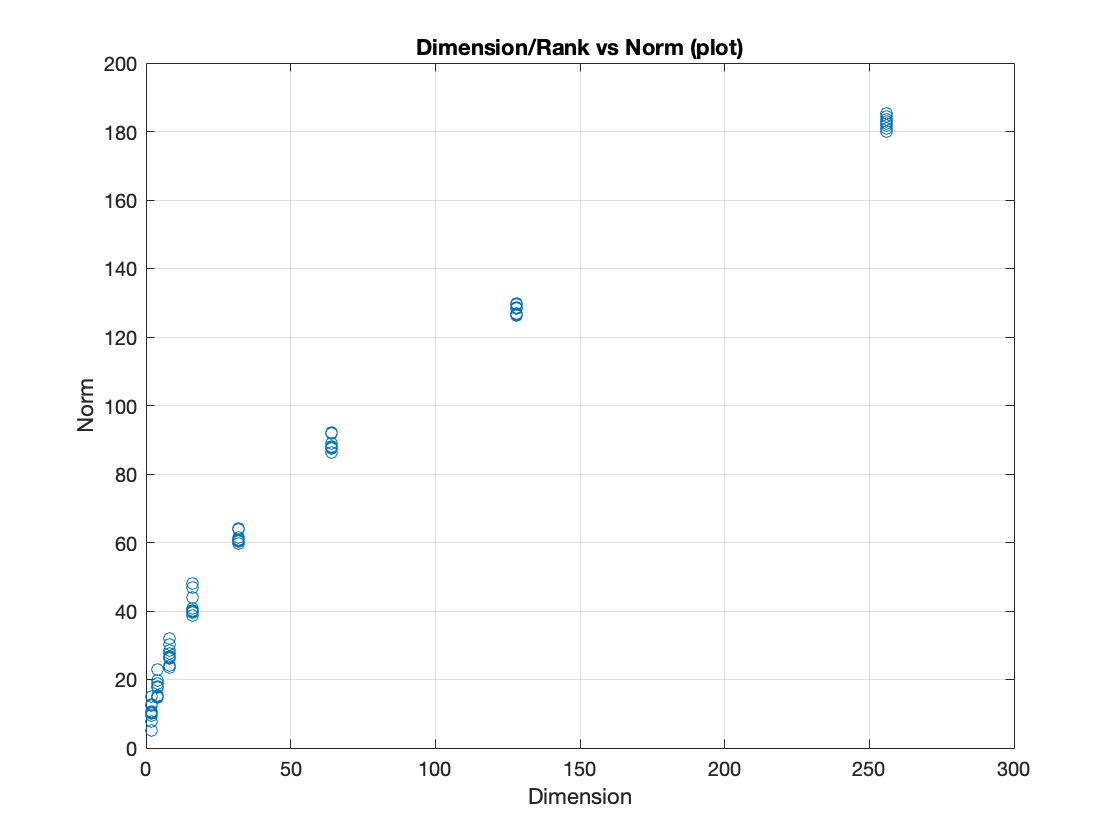
\includegraphics[width= \textwidth]{GenMatrix1.png}
    \end{center}
    \vfill
    \begin{center}
        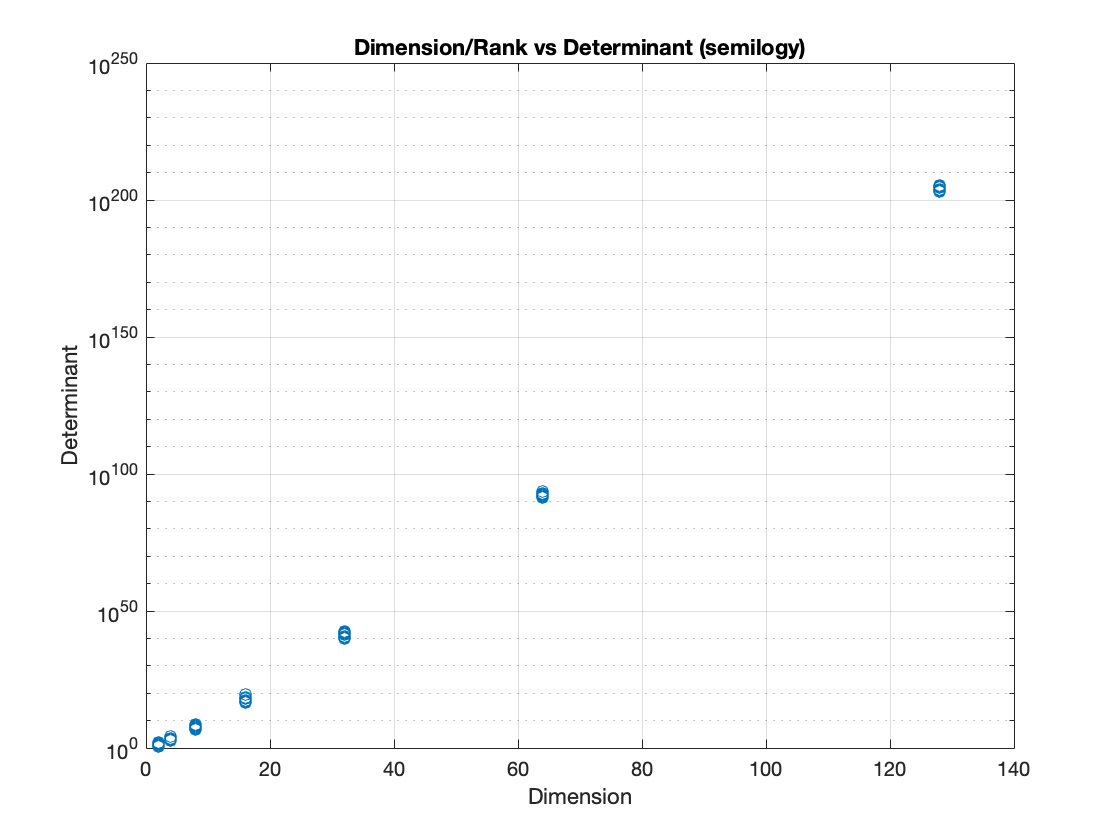
\includegraphics[ width= \textwidth]{GenMatrix2.png}
    \end{center}
    \begin{center}
        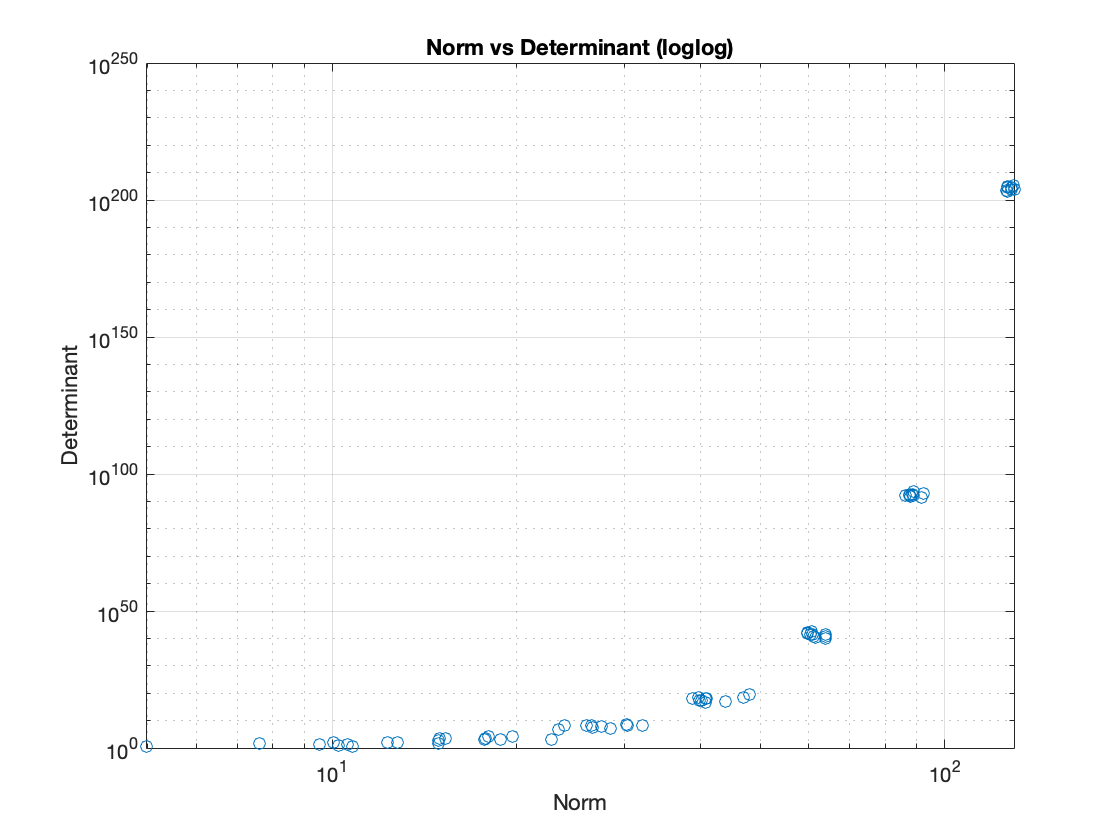
\includegraphics[ width= \textwidth]{GenMatrix3.png}
    \end{center}
    
    

\end{exercise}








\begin{exercise}{3}
    
    \begin{enumerate}
        \item Consider the algorithm which computes the product of a rectangular matrix $A \in \CC^{mxn}$
        ans a column vector $v \in \CC^{n+1}$. Count the number of floating point operations exactly, i.e as an 
        expression in terms of $m$ and $n$.\\

        \solution Recall the definition of matrix vector multiplication, denoted as 1.2 in the reading
        \begin{equation*}
            b = Av = \sum_{i = 1}^n v_ia_i
        \end{equation*}
        Note that A is an mxn matrix and $a_i$ denotes the $i^{th}$ column of the matrix $A$. Since each $a_i$
        has $m$ terms, each $v_ia_i$ term contains $m$ multiplications. Over all $n$ columns there are $mn$ multiplications. 
        Similarly, since there are only $n-1$ additions described in the sum, and each $a_i$ column has $m$ terms there are a total
        of $m(n-1)$ additions. In summation with $mn$ multiplications and $m(n-1)$ additions we get the following, 
        \begin{equation*}
            Total_{FLOPS} = mn + m(n-1) = m(2n-1) 
        \end{equation*}
        \vspace{.25in}
        \item Implement the algorithm in a program $matvec.m$ to multiply a matrix $A$ and vector $v$, include 
        error checking. Test your implementation against Matlab. \\
        \textbf{Code:}
		\begin{center}
			\lstinputlisting{MatVec.m}
		\end{center}

        \textbf{Terminal:}
		\begin{center}
			\lstinputlisting{MatVec1.txt}
		\end{center}
        \vspace{.25in}


        \item Write a function $matmat.m$ for the product $C = AB$ of matrices $A \in \RR^{mxn}$ and
        $B \in \RR^{nxk}$. Count the number of operations. Check your code against the Matlab results for 
        some example $m = 3$, $n = 4$, and $k = 3$.\\
        \solution If we consider the columns of $B$ as individual vectors we get the following idea,
        \begin{equation*}
            AB = A[b_1 | b_2 | ... | b_k] = [Ab_1 | Ab_2 | ... | Ab_k].
        \end{equation*}
        Note that $A$ is an $mxn$ matrix and each column vector $b_i$ is $1xn$. Recall from the previous problem that 
        the total number of flops for a matrix-vector product is,
        \begin{equation*}
            m(2n-1).
        \end{equation*}
        Since it takes $k$ matrix-vector products to produce $AB$ we know that, 
        \begin{equation*}
            Total_{FLOPS} = km(2n-1).
        \end{equation*}
        \textbf{Code:}
		\begin{center}
			\lstinputlisting{MatMat.m}
		\end{center}
        \textbf{Terminal:}
		\begin{center}
			\lstinputlisting{MatMat1.txt}
		\end{center}
    \end{enumerate}
\end{exercise}







\begin{exercise}{4} Let $B$ be any $4x4$ matrix to which we apply the following operations in turn:
    \begin{enumerate}
        \item Interchange rows 1 and 3;
        \begin{equation*}
            \begin{bmatrix}
                0 & 0 & 1 & 0\\
                0 & 1 & 0 & 0\\
                1 & 0 & 0 & 0\\
                0 & 0 & 0 & 1\\
            \end{bmatrix}
            B
        \end{equation*}
        \item Interchange Columns 2 and 4;
        \begin{equation*}
            \begin{bmatrix}
                0 & 0 & 1 & 0\\
                0 & 1 & 0 & 0\\
                1 & 0 & 0 & 0\\
                0 & 0 & 0 & 1\\
            \end{bmatrix}
            B
            \begin{bmatrix}
                1 & 0 & 0 & 0\\
                0 & 0 & 0 & 1\\
                0 & 0 & 1 & 0\\
                0 & 1 & 0 & 0\\
            \end{bmatrix}
        \end{equation*}
        \item Double column 3;
        \begin{equation*}
            \begin{bmatrix}
                0 & 0 & 1 & 0\\
                0 & 1 & 0 & 0\\
                1 & 0 & 0 & 0\\
                0 & 0 & 0 & 1\\
            \end{bmatrix}
            B
            \begin{bmatrix}
                1 & 0 & 0 & 0\\
                0 & 0 & 0 & 1\\
                0 & 0 & 1 & 0\\
                0 & 1 & 0 & 0\\
            \end{bmatrix}
            \begin{bmatrix}
                1 & 0 & 0 & 0\\
                0 & 1 & 0 & 0\\
                0 & 0 & 2 & 0\\
                0 & 0 & 0 & 1\\
            \end{bmatrix}
        \end{equation*}
        \item Add row 3 to row 1;
        \begin{equation*}
            \begin{bmatrix}
                1 & 0 & 1 & 0\\
                0 & 1 & 0 & 0\\
                0 & 0 & 1 & 0\\
                0 & 0 & 0 & 1\\
            \end{bmatrix}
            \begin{bmatrix}
                0 & 0 & 1 & 0\\
                0 & 1 & 0 & 0\\
                1 & 0 & 0 & 0\\
                0 & 0 & 0 & 1\\
            \end{bmatrix}
            B
            \begin{bmatrix}
                1 & 0 & 0 & 0\\
                0 & 0 & 0 & 1\\
                0 & 0 & 1 & 0\\
                0 & 1 & 0 & 0\\
            \end{bmatrix}
            \begin{bmatrix}
                1 & 0 & 0 & 0\\
                0 & 1 & 0 & 0\\
                0 & 0 & 2 & 0\\
                0 & 0 & 0 & 1\\
            \end{bmatrix}
        \end{equation*}
        \item Subtract row 2 from each of the other rows
        \begin{equation*}
            \begin{bmatrix}
                1 & -1 & 0 & 0\\
                0 & 1 & 0 & 0\\
                0 & -1 & 1 & 0\\
                0 & -1 & 0 & 1\\
            \end{bmatrix}
            \begin{bmatrix}
                1 & 0 & 1 & 0\\
                0 & 1 & 0 & 0\\
                0 & 0 & 1 & 0\\
                0 & 0 & 0 & 1\\
            \end{bmatrix}
            \begin{bmatrix}
                0 & 0 & 1 & 0\\
                0 & 1 & 0 & 0\\
                1 & 0 & 0 & 0\\
                0 & 0 & 0 & 1\\
            \end{bmatrix}
            B
            \begin{bmatrix}
                1 & 0 & 0 & 0\\
                0 & 0 & 0 & 1\\
                0 & 0 & 1 & 0\\
                0 & 1 & 0 & 0\\
            \end{bmatrix}
            \begin{bmatrix}
                1 & 0 & 0 & 0\\
                0 & 1 & 0 & 0\\
                0 & 0 & 2 & 0\\
                0 & 0 & 0 & 1\\
            \end{bmatrix}
        \end{equation*}
        \item Replace column 3 with column 4;
        \begin{equation*}
            \begin{bmatrix}
                1 & -1 & 0 & 0\\
                0 & 1 & 0 & 0\\
                0 & -1 & 1 & 0\\
                0 & -1 & 0 & 1\\
            \end{bmatrix}
            \begin{bmatrix}
                1 & 0 & 1 & 0\\
                0 & 1 & 0 & 0\\
                0 & 0 & 1 & 0\\
                0 & 0 & 0 & 1\\
            \end{bmatrix}
            \begin{bmatrix}
                0 & 0 & 1 & 0\\
                0 & 1 & 0 & 0\\
                1 & 0 & 0 & 0\\
                0 & 0 & 0 & 1\\
            \end{bmatrix}
            B
            \begin{bmatrix}
                1 & 0 & 0 & 0\\
                0 & 0 & 0 & 1\\
                0 & 0 & 1 & 0\\
                0 & 1 & 0 & 0\\
            \end{bmatrix}
            \begin{bmatrix}
                1 & 0 & 0 & 0\\
                0 & 1 & 0 & 0\\
                0 & 0 & 2 & 0\\
                0 & 0 & 0 & 1\\
            \end{bmatrix}
            \begin{bmatrix}
                1 & 0 & 0 & 0\\
                0 & 1 & 0 & 0\\
                0 & 0 & 0 & 0\\
                0 & 0 & 1 & 1\\
            \end{bmatrix}
        \end{equation*}
        \item Delete row 1;
        \begin{equation*}
            \begin{bmatrix}
                0 & 1 & 0 & 0\\
                0 & 0 & 1 & 0\\
                0 & 0 & 0 & 1
            \end{bmatrix}
            \begin{bmatrix}
                1 & -1 & 0 & 0\\
                0 & 1 & 0 & 0\\
                0 & -1 & 1 & 0\\
                0 & -1 & 0 & 1\\
            \end{bmatrix}
            \begin{bmatrix}
                1 & 0 & 1 & 0\\
                0 & 1 & 0 & 0\\
                0 & 0 & 1 & 0\\
                0 & 0 & 0 & 1\\
            \end{bmatrix}
            \begin{bmatrix}
                0 & 0 & 1 & 0\\
                0 & 1 & 0 & 0\\
                1 & 0 & 0 & 0\\
                0 & 0 & 0 & 1\\
            \end{bmatrix}
            B
            \begin{bmatrix}
                1 & 0 & 0 & 0\\
                0 & 0 & 0 & 1\\
                0 & 0 & 1 & 0\\
                0 & 1 & 0 & 0\\
            \end{bmatrix}
            \begin{bmatrix}
                1 & 0 & 0 & 0\\
                0 & 1 & 0 & 0\\
                0 & 0 & 2 & 0\\
                0 & 0 & 0 & 1\\
            \end{bmatrix}
            \begin{bmatrix}
                1 & 0 & 0 & 0\\
                0 & 1 & 0 & 0\\
                0 & 0 & 0 & 0\\
                0 & 0 & 1 & 1\\
            \end{bmatrix}
        \end{equation*}
        \item Simplify the product so it becomes a product of 3 matrices $ABC$ where $B$ is the same. \\
        \solution Using the commutativity of matrix multiplication we can work from the inside out to simplify the product. 
        \begin{align*}
            A = 
            \begin{bmatrix}
                0 & 1 & 0 & 0\\
                0 & 0 & 1 & 0\\
                0 & 0 & 0 & 1
            \end{bmatrix}
            &
            \begin{bmatrix}
                1 & -1 & 0 & 0\\
                0 & 1 & 0 & 0\\
                0 & -1 & 1 & 0\\
                0 & -1 & 0 & 1\\
            \end{bmatrix}
            \begin{bmatrix}
                1 & 0 & 1 & 0\\
                0 & 1 & 0 & 0\\
                0 & 0 & 1 & 0\\
                0 & 0 & 0 & 1\\
            \end{bmatrix}
            \begin{bmatrix}
                0 & 0 & 1 & 0\\
                0 & 1 & 0 & 0\\
                1 & 0 & 0 & 0\\
                0 & 0 & 0 & 1\\
            \end{bmatrix}\\
            A = 
            \begin{bmatrix}
                0 & 1 & 0 & 0\\
                0 & 0 & 1 & 0\\
                0 & 0 & 0 & 1
            \end{bmatrix}
            &
            \begin{bmatrix}
                1 & -1 & 0 & 0\\
                0 & 1 & 0 & 0\\
                0 & -1 & 1 & 0\\
                0 & -1 & 0 & 1\\
            \end{bmatrix}
            \begin{bmatrix}
                1 & 0 & 1 & 0\\
                0 & 1 & 0 & 0\\
                1 & 0 & 0 & 0\\
                0 & 0 & 0 & 1\\
            \end{bmatrix}\\
            A = 
            \begin{bmatrix}
                0 & 1 & 0 & 0\\
                0 & 0 & 1 & 0\\
                0 & 0 & 0 & 1
            \end{bmatrix}
            &
            \begin{bmatrix}
                1 & -1 & 1 & 0\\
                0 & 1 & 0 & 0\\
                1 & -1 & 0 & 0\\
                0 & -1 & 0 & 1\\
            \end{bmatrix}\\
            A = 
            \begin{bmatrix}
                0 & 1 & 0 & 0\\
                1 & -1 & 0 & 0\\
                0 & -1 & 0 & 1\\
            \end{bmatrix}
        \end{align*}
        Similarly we can compute $C$, 
        \begin{align*}
            C = 
            \begin{bmatrix}
                1 & 0 & 0 & 0\\
                0 & 0 & 0 & 1\\
                0 & 0 & 1 & 0\\
                0 & 1 & 0 & 0\\
            \end{bmatrix}
            &
            \begin{bmatrix}
                1 & 0 & 0 & 0\\
                0 & 1 & 0 & 0\\
                0 & 0 & 2 & 0\\
                0 & 0 & 0 & 1\\
            \end{bmatrix}
            \begin{bmatrix}
                1 & 0 & 0 & 0\\
                0 & 1 & 0 & 0\\
                0 & 0 & 1 & 1\\
                0 & 0 & 0 & 0\\
            \end{bmatrix}\\
            C = 
            \begin{bmatrix}
                1 & 0 & 0 & 0\\
                0 & 0 & 0 & 1\\
                0 & 0 & 2 & 0\\
                0 & 1 & 0 & 0\\
            \end{bmatrix}
            &
            \begin{bmatrix}
                1 & 0 & 0 & 0\\
                0 & 1 & 0 & 0\\
                0 & 0 & 0 & 0\\
                0 & 0 & 1 & 1\\
            \end{bmatrix}\\
            C = 
            \begin{bmatrix}
                1 & 0 & 0 & 0\\
                0 & 0 & 1 & 1\\
                0 & 0 & 0 & 0\\
                0 & 1 & 0 & 0\\
            \end{bmatrix}
        \end{align*}
        Finally we get that, 
        \begin{equation*} 
        \begin{bmatrix}
            0 & 1 & 0 & 0\\
            1 & -1 & 0 & 0\\
            0 & -1 & 0 & 1\\
        \end{bmatrix}
        B
        \begin{bmatrix}
            1 & 0 & 0 & 0\\
            0 & 0 & 1 & 1\\
            0 & 0 & 0 & 0\\
            0 & 1 & 0 & 0\\
        \end{bmatrix}
        \end{equation*}
    \end{enumerate}



\end{exercise}


\begin{exercise}{1.3} Generalizing Example 1.3, we say that a square or 
    rectangular matrix $R$ with entries $r_{i,j}$ is upper-triangular if $r_{i,j} = 0$
    for $i>j$. By considering what space is spanned by the first $n$ columns of $R$ and using $(1.8)$, 
    show that if $R$ is a nonsingular $mxm$ upper-triangular matrix, then $R^{-1}$ is also upper triangular. \\
    \solution Suppose that if $R$ is a nonsingular $mxm$ upper-triangular matrix. Note that by definition $R$ is 
    a square matrix in row echelon form with no pivot values and is therefore full-rank and fully invertible. Consider that by $(1.8)$, 
    \begin{align*}
        RR^{-1} &= I, \\
        R[r^{-1}_1 r^{-1}_2 \dots r^{-1}_m] &= I.
    \end{align*}
    So for some $k \in (1,m)$ we know that, 
    \begin{equation*}
        Rr^{-1}_k = e_k.
    \end{equation*}
    Note that since $e_k$ has all zeros below the $k^{th}$ row we know that the same must be true for $r^{-1}_k$,
    since $R$ is lower triangular, a non zero value below the $k^{th}$ row of $r^{-1}_k$ would show up in $e_k$. This property extends to 
    all columns in $R^{-1}$ and therefore $R^{-1}$ must be upper triangular. 



\end{exercise}


\end{document}




















